\section{Experiment}
\subsection{Dataset and Setup}
This work targets the 6082 aluminum alloy control-arm forging and constructs a dataset of 600 forging simulations based on DEFORM-3D, in which both the initial temperature field and the forging speed vary, and each sequence contains 67 deformation steps. Ten non-uniform initial temperature fields are obtained by simulating the cooling process. Each simulation outputs multi-physics fields such as temperature, von Mises stress, and damage, which are stored as point clouds with about 5000 points per step, each point recording its coordinate $(x,y,z)$ and the corresponding physical quantities; the dataset is split into training, validation, and test sets.
% 【待定：训练/验证/测试划分比例】

For preprocessing, the absolute coordinates of all points are normalized along the three axes with a shared scale to preserve the workpiece shape.

The main hyperparameters are set as follows: number of points per step $N=5000$, latent-state dimension $d=48$, and encoder level count $n_{\text{SA}}=4$. The critical damage value of the damage constraint is set to $D_{\text{cr}}=0.43$.
% 【待补：其余超参数与实验环境】

\subsection{World Model Evaluation}

The world model is trained in two stages. Fig.~\ref{fig:train_loss} shows the training loss curves of the two stages: the first stage trains the encoder and decoder with the reconstruction loss (Fig.~\ref{fig:train_loss_a}), and the second stage trains the latent dynamics model with the prediction loss (Fig.~\ref{fig:train_loss_b}). The training and validation losses of both stages decrease and stabilize over epochs, converging synchronously with a stable gap and no evident overfitting, indicating that both the reconstruction representation and the latent-space dynamics have effectively converged.

\begin{figure}[H]
    \centering
    \subfloat[Stage 1 (reconstruction)]{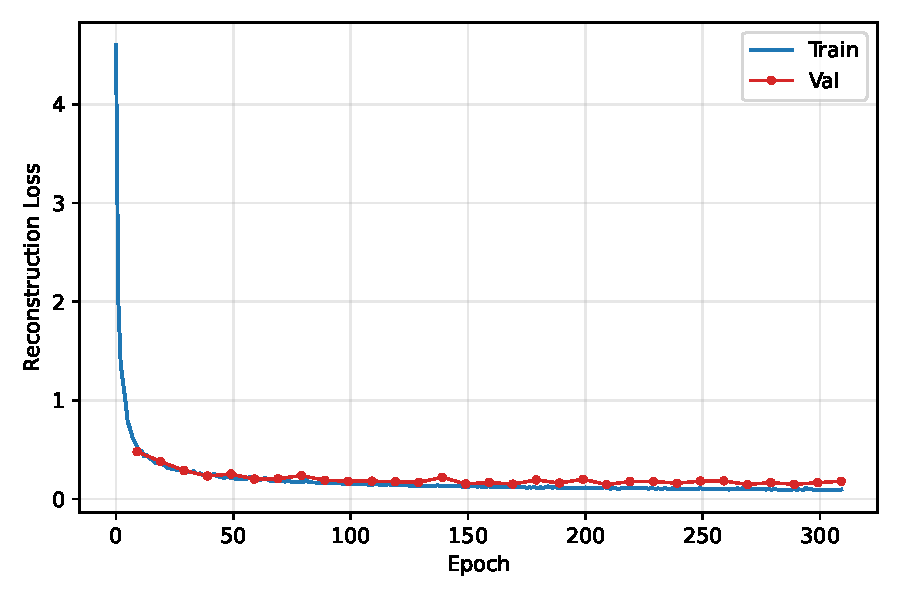
\includegraphics[width=0.44\linewidth]{train_loss_1.pdf}\label{fig:train_loss_a}}
    \qquad
    \subfloat[Stage 2 (prediction)]{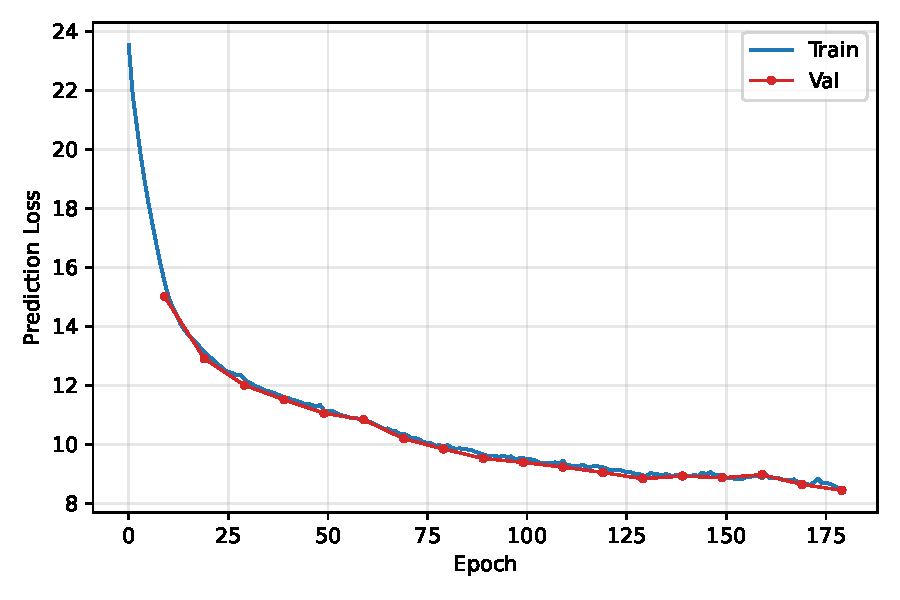
\includegraphics[width=0.44\linewidth]{train_loss_2.pdf}\label{fig:train_loss_b}}
    \caption{Loss curves of the two-stage training of the world model.}
    \label{fig:train_loss}
\end{figure}

To evaluate the prediction accuracy of the world model, taking the stress field as an example, its predictions are compared with the finite element (FE) simulation and the baseline method. Fig.~\ref{fig:model_result} shows the stress-field point clouds at five deformation steps along the deformation history: the first row is the FE ground truth, the second row is the prediction of the proposed model, and the third row is the result of the DeepONet baseline. The stress distribution of the proposed model is highly consistent with the ground truth, with the deviation concentrated in local regions and of small magnitude; the baseline exhibits a clear distribution shift in the stress-concentration regions.

\begin{figure}[H]
\centerline{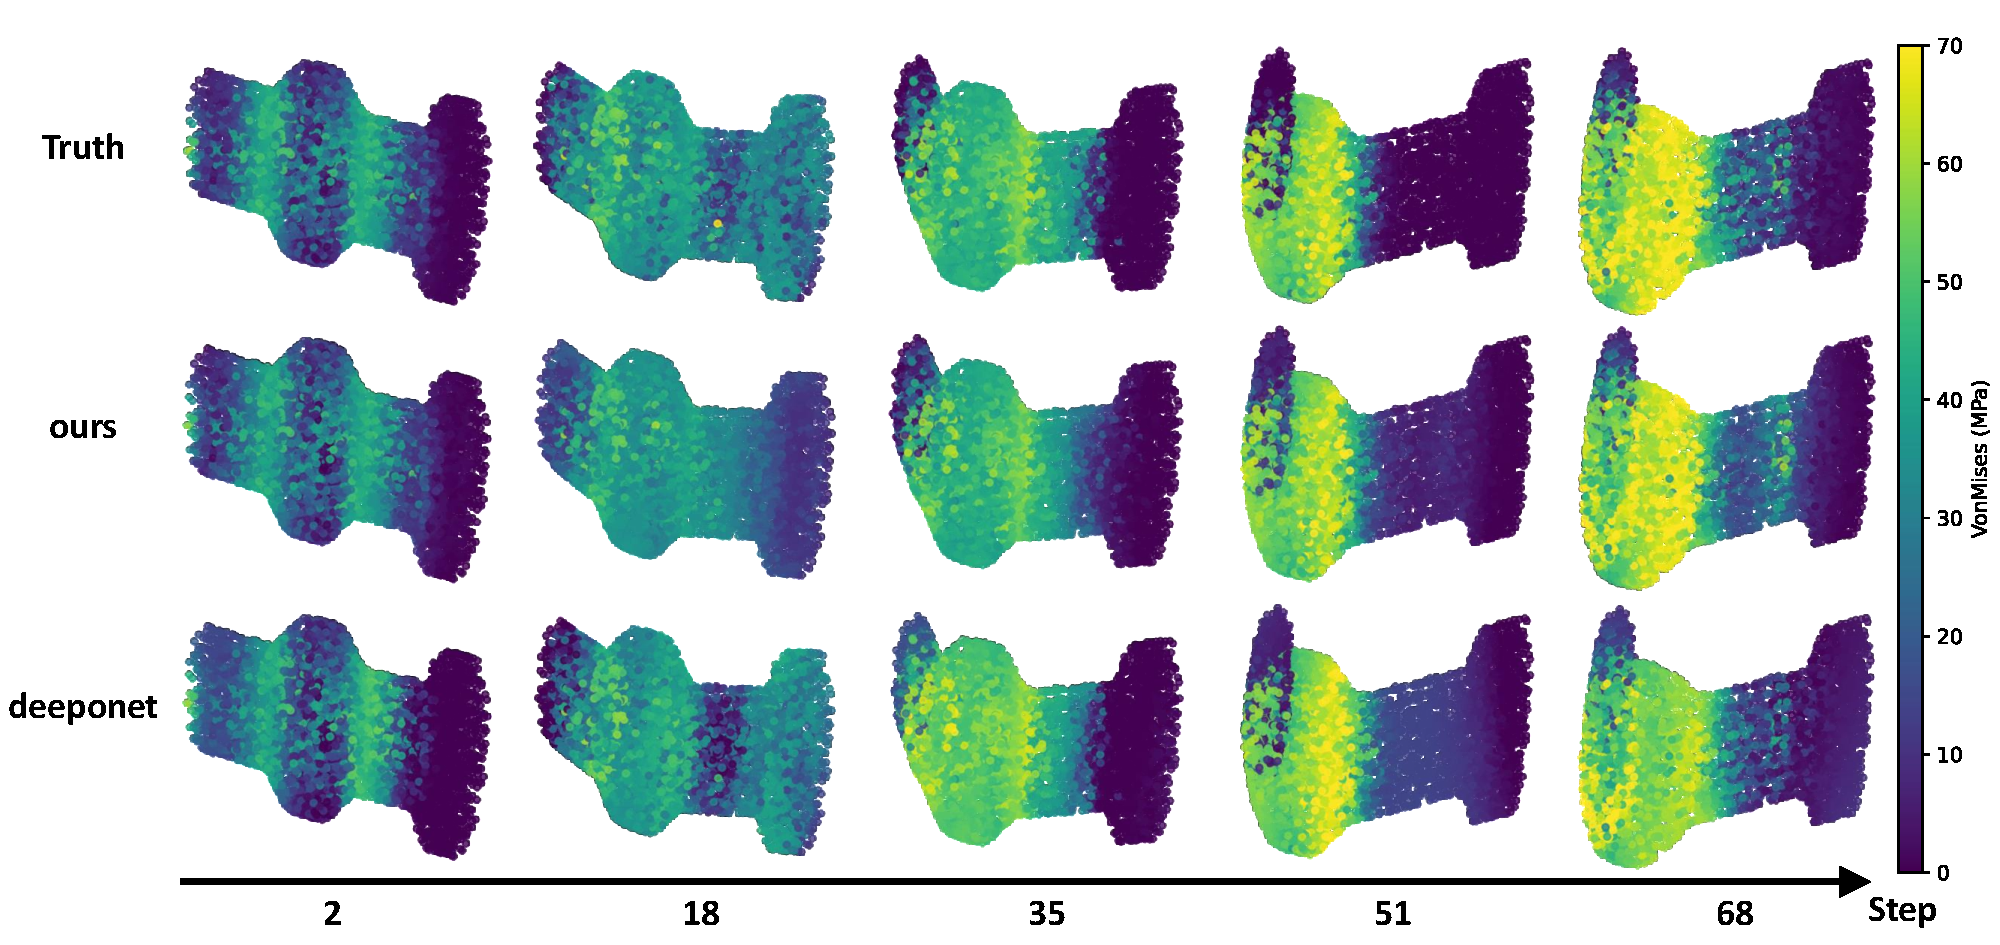
\includegraphics[width=9cm]{timeline-1.pdf}}
\caption{Stress-field prediction comparison: the three rows, from top to bottom, are the FE ground truth, the prediction of the proposed model, and the DeepONet baseline; each row shows the point clouds at five deformation steps along the deformation history from left to right.}
\label{fig:model_result}
\end{figure}

Errors are further quantified on the test set. At inference, the trained latent dynamics model integrates along the stroke to propagate, and the decoder reconstructs the point cloud. The geometry error is reported as per-axis root mean square error (RMSE) in mm, and the physical-field errors are normalized by the mean and variance of each field on the training set, computed per channel and then averaged, with the errors compared pointwise with the corresponding FE results. Under this rollout manner, the per-axis geometry RMSE is 1.63 mm, and the averaged normalized MSE over the three physical fields is 0.080; the per-channel results are shown in Table~\ref{tab:model_error}. Among the three channels, the von Mises stress has the highest normalized error, followed by temperature and then damage. The von Mises stress is jointly determined by the strain rate and temperature and depends on the entire deformation history, making it the most sensitive to process conditions among the three fields; temperature is dominated by heat conduction with a smooth distribution and is relatively easier to fit; damage accumulates only locally with most points close to zero, so the pointwise error is diluted by a large number of near-zero points and its normalized error is the lowest. The decision stage requires repeatedly rolling out the entire curve within the world model, thereby supporting stepwise decision-making.

\begin{table}[H]
\centering
\caption{Prediction errors of the proposed and baseline methods}
\label{tab:model_error}
\setlength{\tabcolsep}{5pt}
\footnotesize
\begin{tabular}{l c c c c c}
\toprule
 & RMSE (mm) & \multicolumn{4}{c}{Normalized MSE} \\
Model & Geometry & Temp. & von Mises & Dmg. & avg. \\
\midrule
Ours & 1.63 & 0.104 & 0.115 & 0.022 & 0.080 \\
DeepONet (no latent) & 1.57 & 0.129 & 0.255 & 0.031 & 0.138 \\
\bottomrule
\end{tabular}

\vspace{2pt}
{\footnotesize Note: geometry is per-axis RMSE (mm); field normalized MSE uses training-set statistics; avg.\ is the mean over the three field channels; all metrics are averaged over the test-set rollout. Full-model physical RMSE: 8.8\,$^{\circ}$C, 6.3 MPa, $4.7\times10^{-3}$ (temperature, von Mises, damage).}
\end{table}

The same-metric errors on the training set are 1.87 mm for geometry, 9.7\,$^{\circ}$C for temperature, 7.9 MPa for von Mises stress, and $5.6\times10^{-3}$ for damage, slightly higher than on the test set. The reason is that the training set covers a wider range of temperature and deformation, and the normalization statistics are taken from the training set; the errors of the two sets are of the same order and the deviations of each channel are in the same direction, with no overfitting sign that the training set is significantly better than the test set.




\subsection{Decision Results}
The average reward and damage during the training of the policy are shown in Fig.~\ref{fig:combined_curves}. The average reward rises from initial fluctuations and stabilizes at a positive value (Fig.~\ref{fig:reward_a}), indicating that the policy has converged; Fig.~\ref{fig:damage_b} shows the maximum damage over the whole process in each epoch, which stabilizes below the critical value $D_{\text{cr}}$ in the late training stage. Since the maximum has not exceeded the limit, no step has exceeded the limit, and the stepwise constraint is thereby satisfied. These results show that the proposed decision method shortens the forging time while satisfying the damage constraint.

\begin{figure}[H]
    \centering
    \subfloat[Reward]{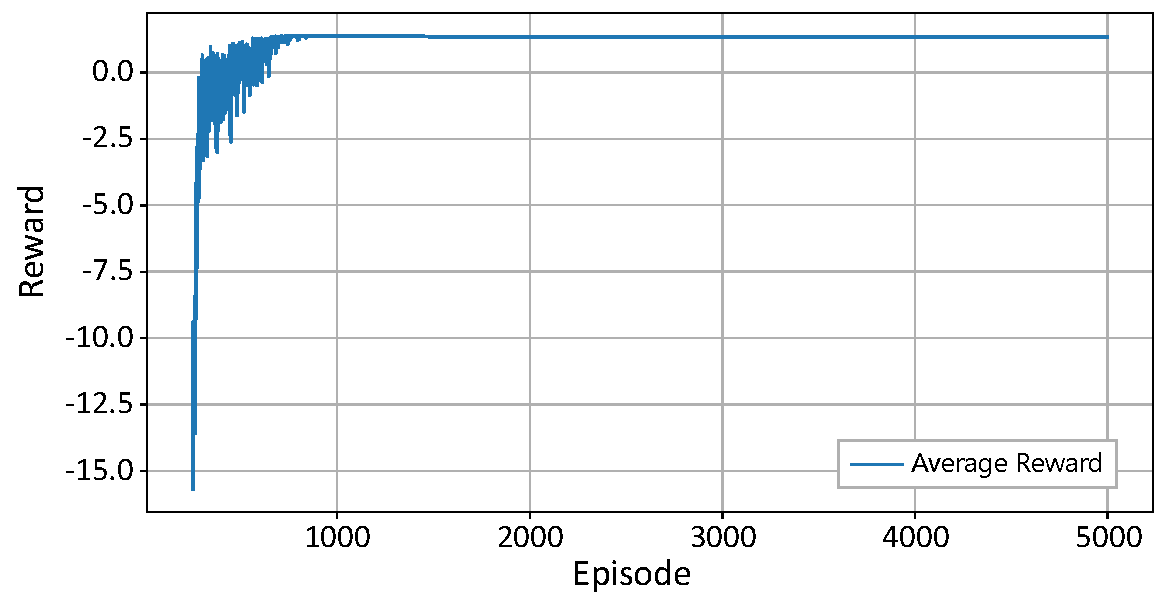
\includegraphics[width=0.38\linewidth]{reward-1.pdf}\label{fig:reward_a}}
    \qquad
    \subfloat[Damage]{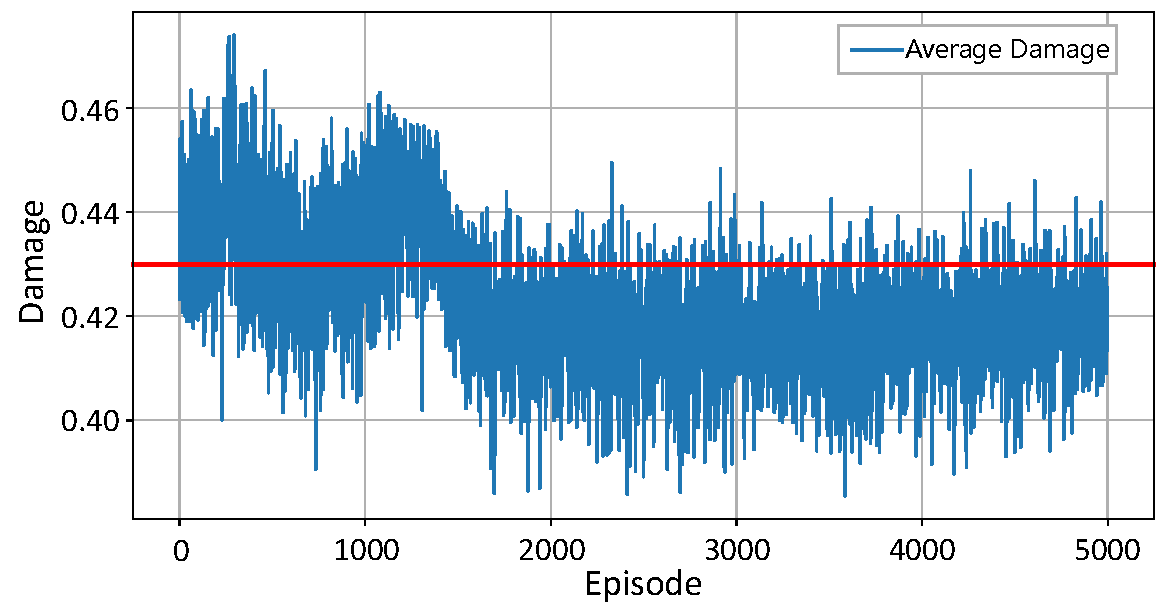
\includegraphics[width=0.38\linewidth]{damage-1.pdf}\label{fig:damage_b}}
    \caption{Training parameter over epochs.}
    \label{fig:combined_curves}
\end{figure}

Fig.~\ref{fig:ours_speed} shows the speed profiles and damage curves generated by the proposed method under different initial temperature fields. When the initial temperature rises from $474\,^{\circ}\mathrm{C}$ to $500\,^{\circ}\mathrm{C}$, the acceleration segment of the speed profile advances and the forging time shortens, indicating that the policy can adaptively adjust the speed profile according to the initial temperature field to exploit the high-temperature softening of the material; the damage curve rises gradually with deformation and reaches its peak at the last step, with its ratio to the critical damage value $D_{\text{cr}}$ still below 1.0, indicating that the damage is overall controlled.

\begin{figure}[H]
    \centering
    \begin{minipage}[t]{0.44\textwidth}
        \centering
        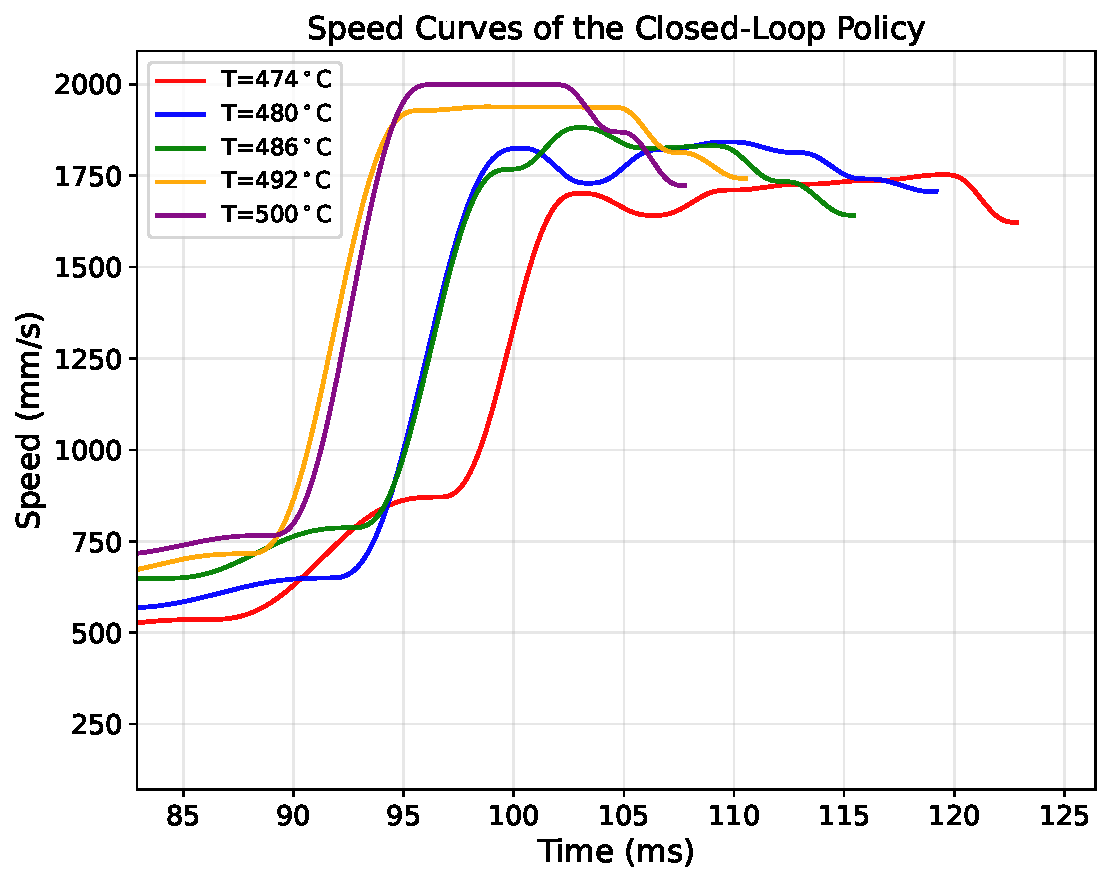
\includegraphics[width=\linewidth]{speed_close.pdf}
        \caption{Speed profiles and damage curves generated by the proposed method under different initial temperature fields ($474\,^{\circ}\mathrm{C}$--$500\,^{\circ}\mathrm{C}$). The damage curve takes the average of the top 50 points with the largest damage in the point cloud at each step.}
        \label{fig:ours_speed}
    \end{minipage}
    \qquad
    \begin{minipage}[t]{0.44\textwidth}
        \centering
        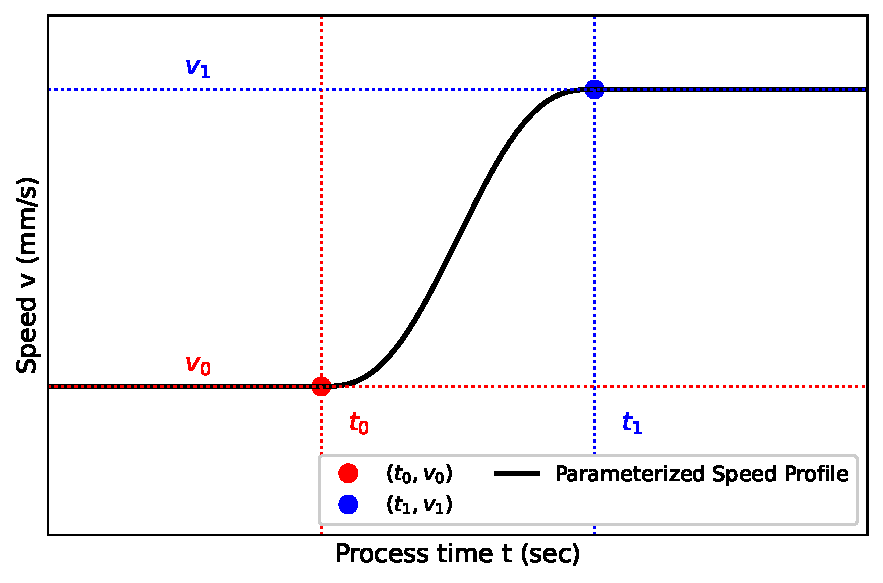
\includegraphics[width=\linewidth]{velocity_profile.pdf}
        \caption{Three-segment shape of the single-shot parametric decision.}
        \label{fig:speed_profile}
    \end{minipage}
\end{figure}

\textbf{Baselines.} The single-shot parametric decision is also a trained parametric policy; its difference from the proposed policy lies in the decision representation: the proposed method outputs the speed of each step step by step, whereas it directly gives a four-dimensional speed parameter $\theta=\{v_0,v_1,t_0,t_1\}$ in a single-shot manner and then reconstructs the entire speed profile from it. The profile is restricted to a ``constant--accelerating--constant'' three-segment shape, given by a smooth four-parameter function:
\begin{equation}
v_{y}(t)=\begin{cases}
v_{0}, & t<t_{0} \\
v_{0}+(v_{1}-v_{0})\,\xi^{3}\,(10-15\xi+6\xi^{2}), & t_{0}\le t\le t_{1} \\
v_{1}, & t>t_{1}
\end{cases}
\end{equation}
where $\xi=(t-t_0)/(t_1-t_0)$, and the components of $\theta$ correspond to the initial speed, the target speed, and the start/end instants of acceleration; this function has second-order continuous derivatives at $t_0$ and $t_1$, ensuring smooth acceleration. The parametric policy takes the initial temperature field as input and outputs $\theta$ in a single shot, with the training objective likewise being to shorten the forging time within the world model while satisfying the damage constraint. Because it does not require stepwise autoregressive generation of the curve, its decision time is lower than that of the proposed method, at the cost of forgoing the stepwise utilization of the evolution process. PSO, in contrast, is not trained; it performs a global search with particle swarm over the same parameter curve, and its decision time mainly comes from repeated fitness evaluations.

\begin{figure}[H]
    \centering
    \subfloat[Single-shot parametric decision]{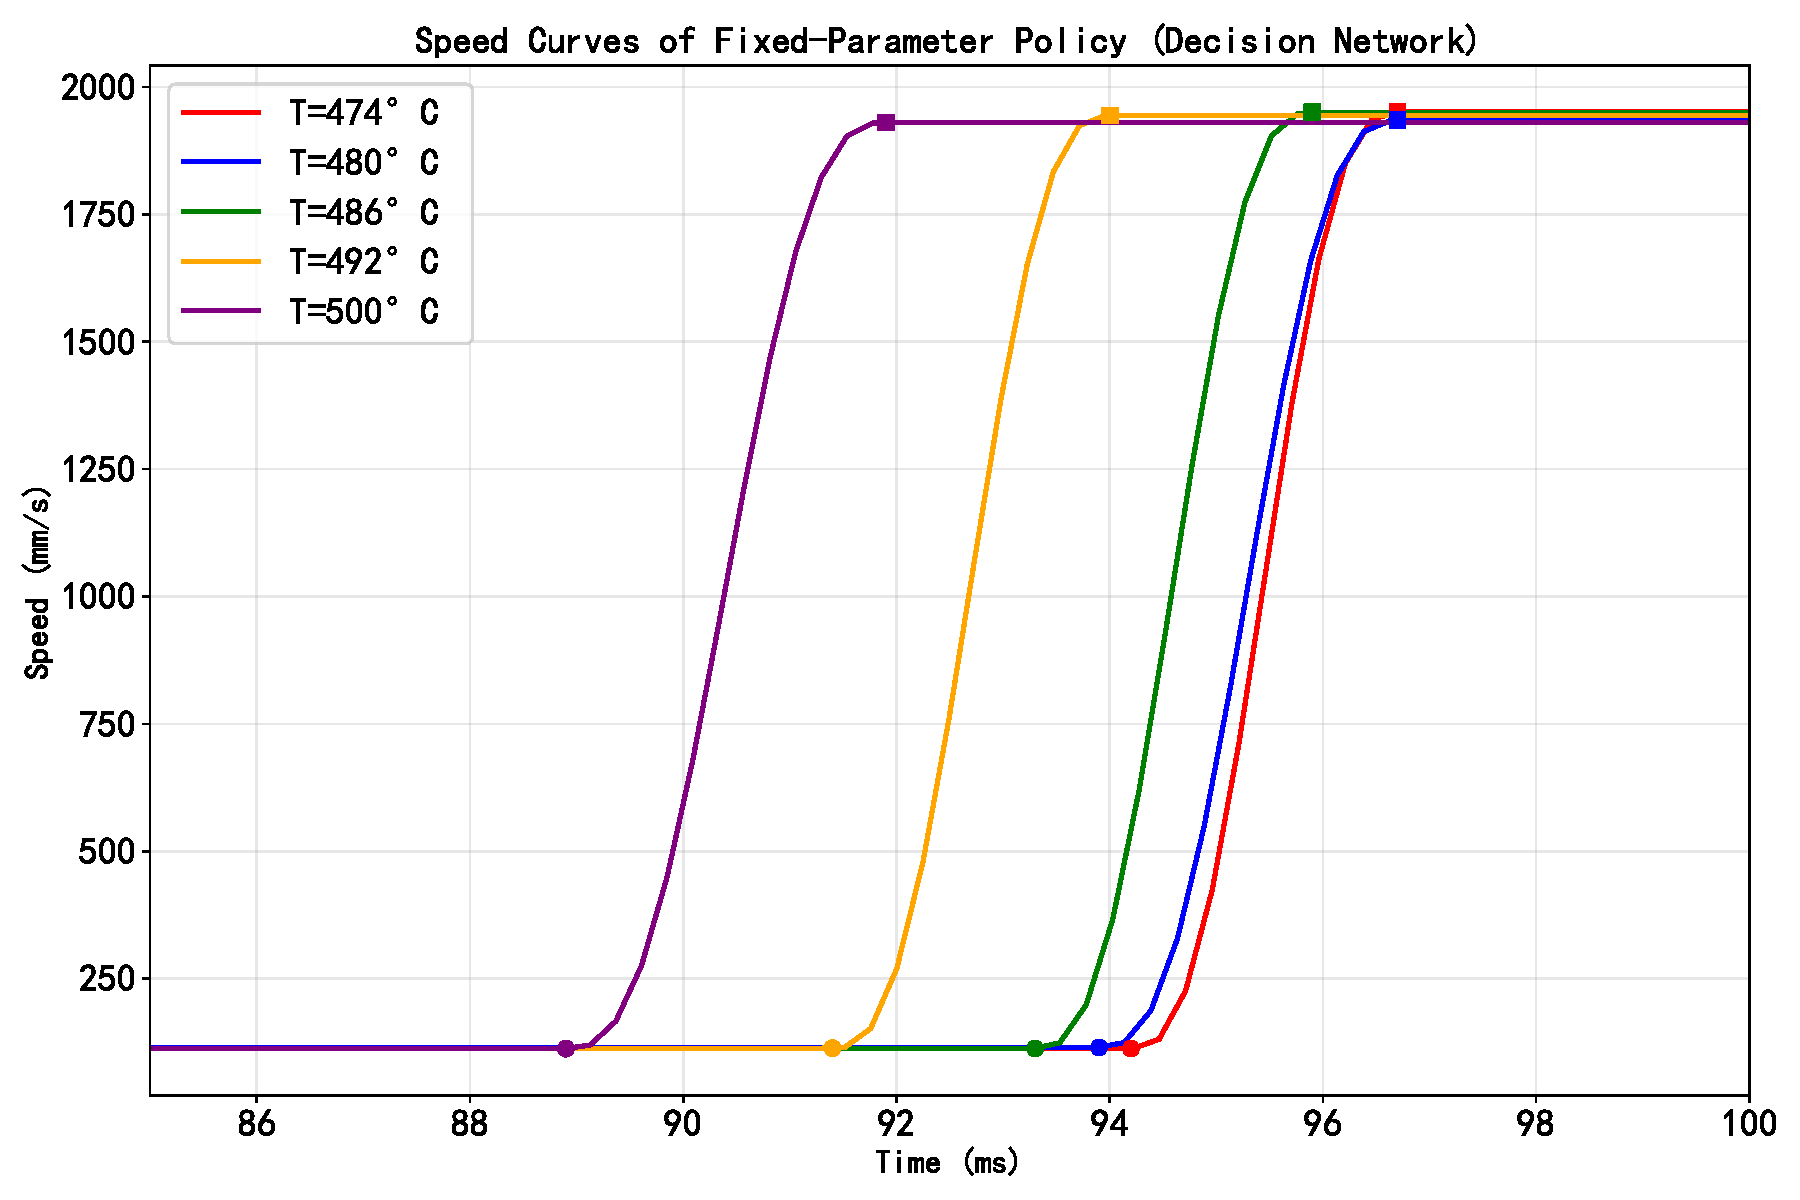
\includegraphics[width=0.40\linewidth]{NetworkSpeed_decision.pdf}\label{fig:policynet_speed}}
    \qquad
    \subfloat[PSO]{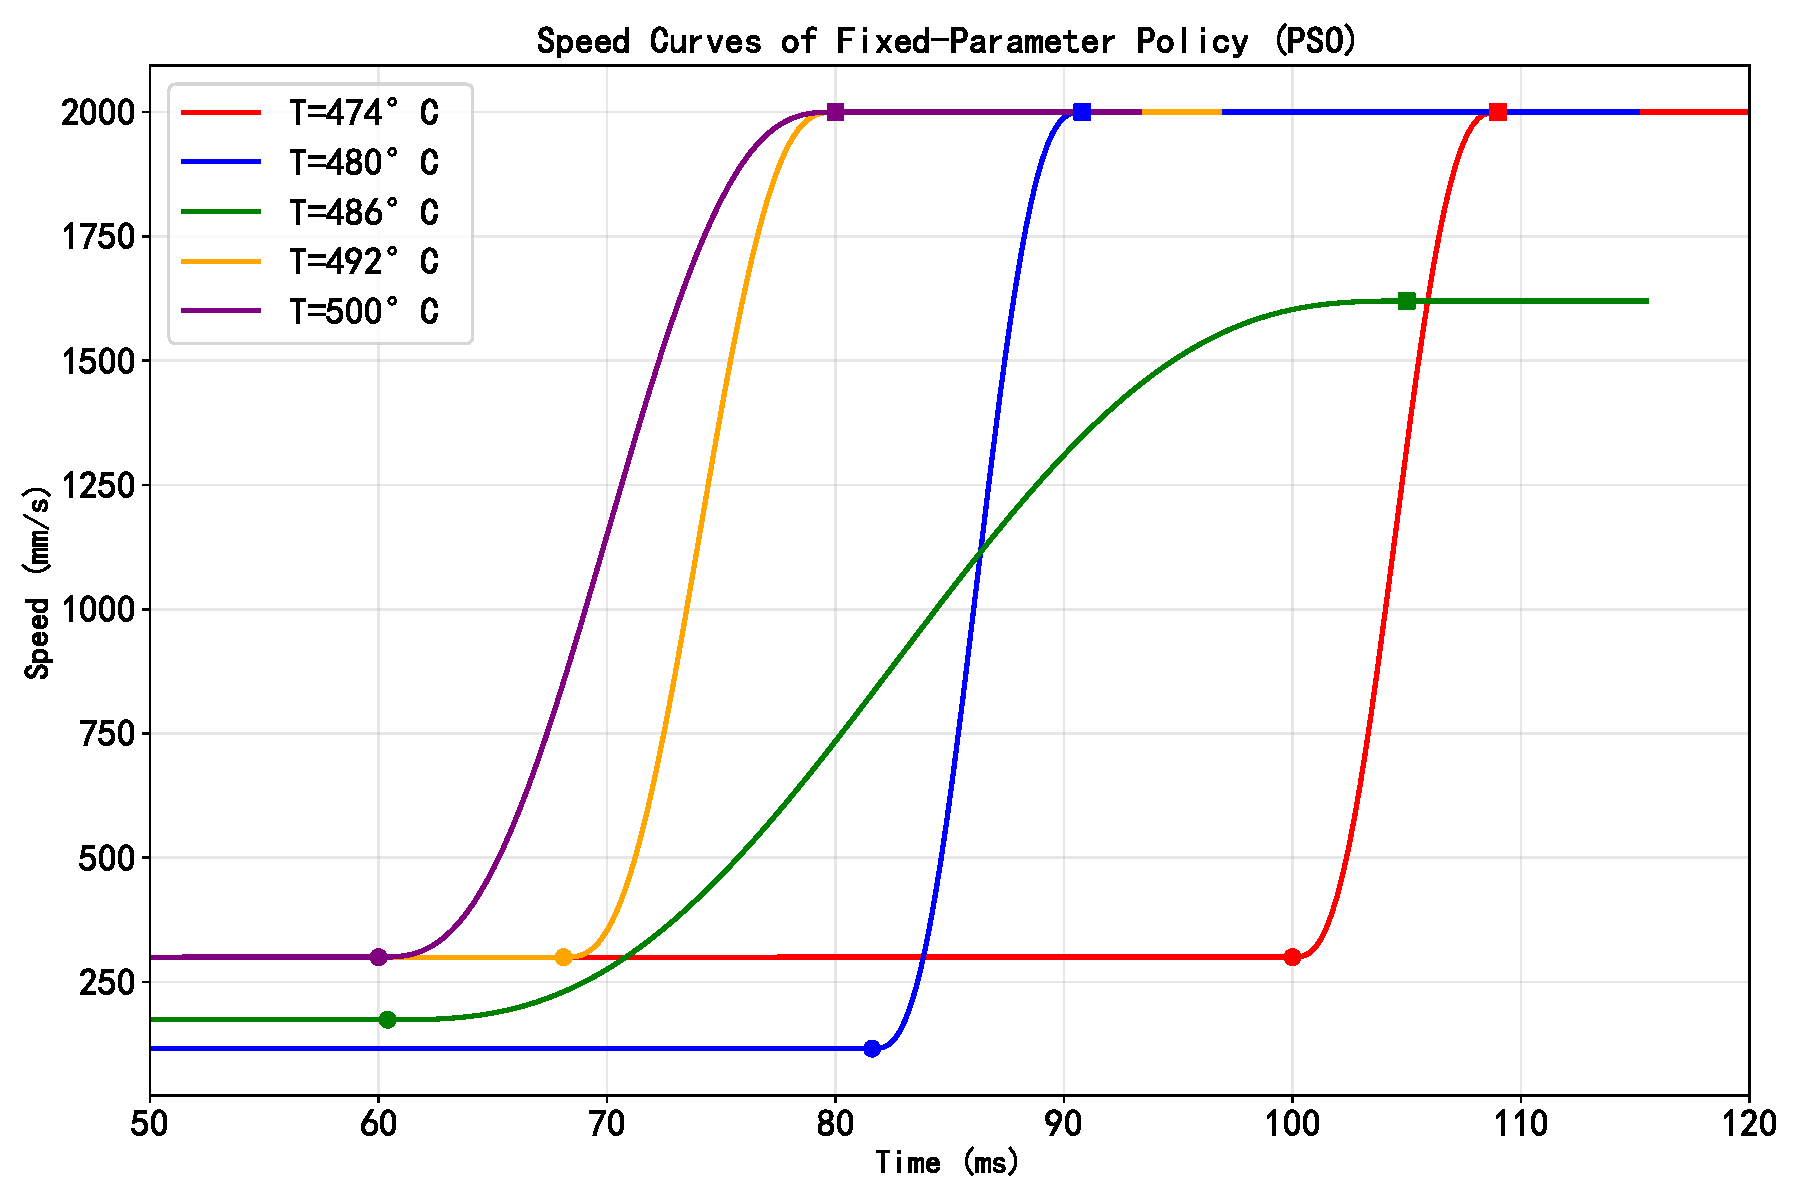
\includegraphics[width=0.40\linewidth]{NetworkSpeed_PSO.pdf}\label{fig:pso_speed}}
    \caption{Speed-profile comparison with other decision methods ($474\,^{\circ}\mathrm{C}$--$500\,^{\circ}\mathrm{C}$).}
    \label{fig:other_speed}
\end{figure}

The process performance and decision efficiency of different decision methods are further compared; the speed profiles of each method are shown in Fig.~\ref{fig:ours_speed} and Fig.~\ref{fig:other_speed}, respectively, and the quantitative results are given in Table~\ref{tab:Method Comparison}. PSO achieves the best process quality, with the shortest forging time and a damage rate of 0, but its solution is time-consuming and cannot meet the requirement of rapid pre-production decision; the single-shot parametric decision has the longest forging time and gives the decision very fast, but damage appears in the simulation and safety cannot be guaranteed; the forging time of the proposed method lies in between, slightly longer than PSO but shorter than the single-shot parametric decision. Its decision is slightly slower than the single-shot parametric decision due to autoregressive stepwise inference, yet still clearly faster than PSO, and no damage appears in the simulation test. It can be seen that the proposed method obtains damage-free safety at a very small cost in forging time, while its forging time is better than the single-shot parametric decision and its decision speed is far better than PSO.

\begin{table}[H]
\centering
\caption{Performance comparison of the three decision methods}
\setlength{\tabcolsep}{3.5pt}
\begin{tabular}{c c c c}
\toprule
\textbf{Method} & \textbf{Forge Time} & \textbf{Decision Time} & \textbf{Damage Rate}\\
& (mean$\pm$std,ms) & (mean$\pm$std,ms) & (\%)\\
\midrule
Ours & 115.14$\pm$6.15 & 105.21$\pm$4.13 & 0.00 \\
Parametric decision & 119.18$\pm$4.84 & 97.37$\pm$3.86 & 8.00 \\
PSO        & 108.72$\pm$11.55 & 2580$\pm$1370 & 0.00 \\
\bottomrule
\end{tabular}
\label{tab:Method Comparison}
\end{table}

The decision time of PSO mainly comes from repeated fitness evaluations. Fig.~\ref{fig:pso_objective} shows the convergence process of its objective function: PSO requires about 0.9 s to optimize to an objective value comparable to the parametric-policy output, and full convergence requires 2580 ms; in contrast, the parametric policy directly gives the speed parameter through a single forward inference without iterative search. Therefore, although the parametric policy does not obtain the optimal solution of PSO, it is significantly superior in time efficiency.

\begin{figure}[H]
\centerline{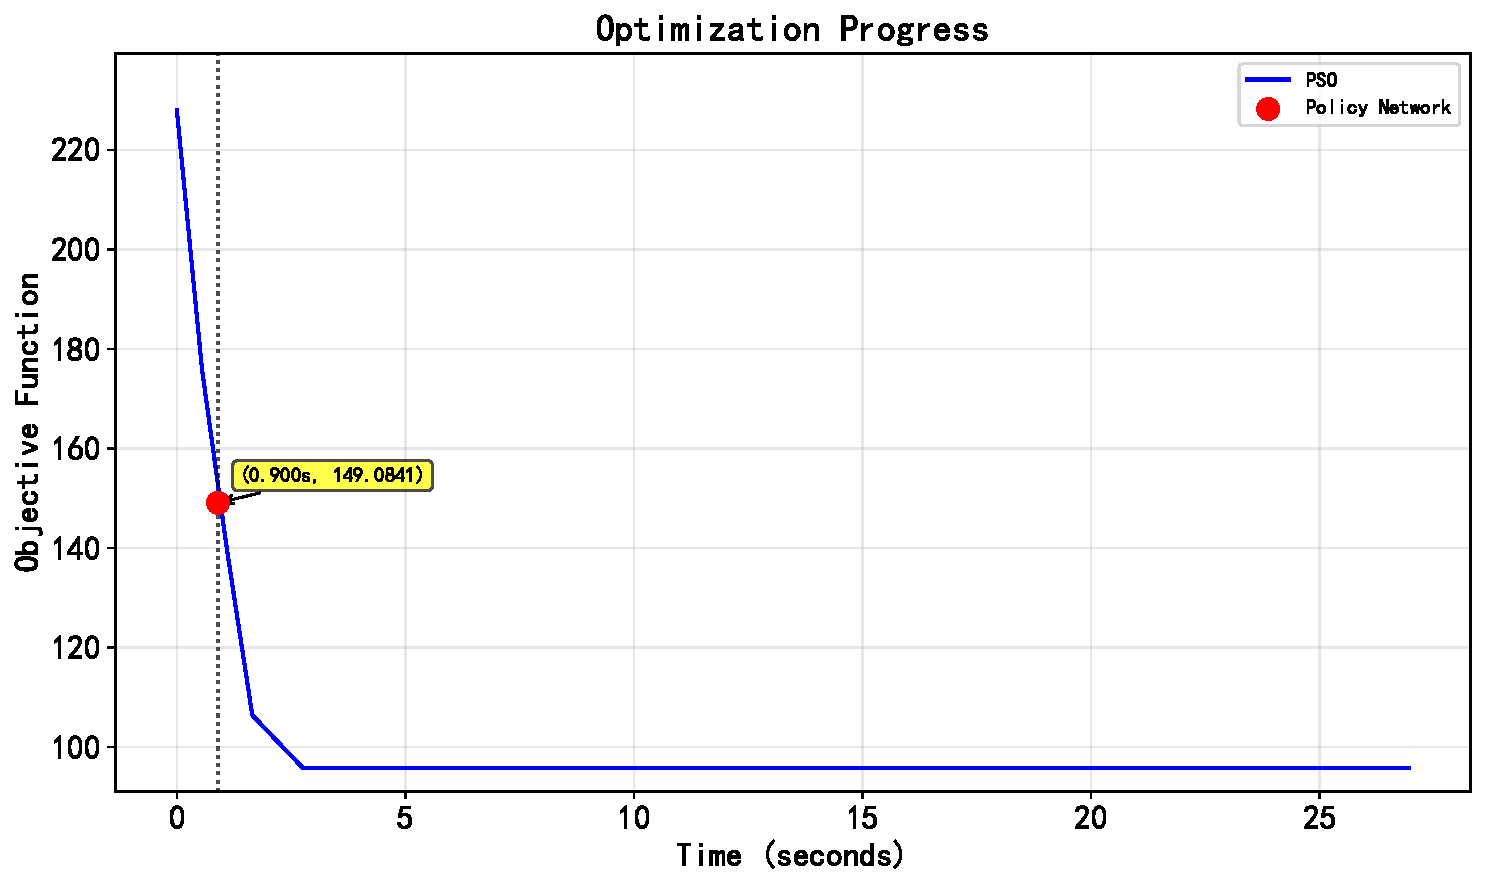
\includegraphics[width=9cm]{PSO-Objective_linear.pdf}}
\caption{Convergence curve of the objective function during PSO solving.}
\label{fig:pso_objective}
\end{figure}

In summary, PSO and the single-shot parametric decision are respectively insufficient in decision efficiency and safety, whereas the proposed method maintains an acceptable forging time and a decision speed far superior to PSO while guaranteeing no damage, and is thus more suitable for practical forging conditions.
